\documentclass[hidelinks,12pt]{article}
\usepackage[left=0.25cm,top=1cm,right=0.25cm,bottom=1cm]{geometry}
%\usepackage[landscape]{geometry}
\textwidth = 20cm
\hoffset = -1cm
\usepackage[utf8]{inputenc}
\usepackage[spanish,es-tabla]{babel}
\usepackage[autostyle,spanish=mexican]{csquotes}
\usepackage[tbtags]{amsmath}
\usepackage{nccmath}
\usepackage{amsthm}
\usepackage{amssymb}
\usepackage{mathrsfs}
\usepackage{graphicx}
\usepackage{subfig}
\usepackage{standalone}
\usepackage[outdir=./Imagenes/]{epstopdf}
\usepackage{siunitx}
\usepackage{physics}
\usepackage{color}
\usepackage{float}
\usepackage{hyperref}
\usepackage{multicol}
%\usepackage{milista}
\usepackage{anyfontsize}
\usepackage{anysize}
%\usepackage{enumerate}
\usepackage[shortlabels]{enumitem}
\usepackage{capt-of}
\usepackage{bm}
\usepackage{relsize}
\usepackage{placeins}
\usepackage{empheq}
\usepackage{cancel}
\usepackage{wrapfig}
\usepackage[flushleft]{threeparttable}
\usepackage{makecell}
\usepackage{fancyhdr}
\usepackage{tikz}
\usepackage{bigints}
\usepackage{scalerel}
\usepackage{pgfplots}
\usepackage{pdflscape}
\pgfplotsset{compat=1.16}
\spanishdecimal{.}
\renewcommand{\baselinestretch}{1.5} 
\renewcommand\labelenumii{\theenumi.{\arabic{enumii}})}
\newcommand{\ptilde}[1]{\ensuremath{{#1}^{\prime}}}
\newcommand{\stilde}[1]{\ensuremath{{#1}^{\prime \prime}}}
\newcommand{\ttilde}[1]{\ensuremath{{#1}^{\prime \prime \prime}}}
\newcommand{\ntilde}[2]{\ensuremath{{#1}^{(#2)}}}

\newtheorem{defi}{{\it Definición}}[section]
\newtheorem{teo}{{\it Teorema}}[section]
\newtheorem{ejemplo}{{\it Ejemplo}}[section]
\newtheorem{propiedad}{{\it Propiedad}}[section]
\newtheorem{lema}{{\it Lema}}[section]
\newtheorem{cor}{Corolario}
\newtheorem{ejer}{Ejercicio}[section]

\newlist{milista}{enumerate}{2}
\setlist[milista,1]{label=\arabic*)}
\setlist[milista,2]{label=\arabic{milistai}.\arabic*)}
\newlength{\depthofsumsign}
\setlength{\depthofsumsign}{\depthof{$\sum$}}
\newcommand{\nsum}[1][1.4]{% only for \displaystyle
    \mathop{%
        \raisebox
            {-#1\depthofsumsign+1\depthofsumsign}
            {\scalebox
                {#1}
                {$\displaystyle\sum$}%
            }
    }
}
\def\scaleint#1{\vcenter{\hbox{\scaleto[3ex]{\displaystyle\int}{#1}}}}
\def\bs{\mkern-12mu}



\title{Teorema de adición de los armónicos esféricos \\ {\large Tema 4 - Separación de variables en coordenadas esféricas}\vspace{-1ex}}
\author{M. en C. Gustavo Contreras Mayén}
\date{ }

\pagestyle{fancy}
\fancyhf{}
\rhead{Curso MAF}
\lhead{\leftmark}
\rfoot{\thepage}
\setlength{\headheight}{16pt}%

\def\changemargin#1#2{\list{}{\rightmargin#2\leftmargin#1}\item[]}
\let\endchangemargin=\endlist 


\begin{document}
\maketitle
\fontsize{14}{14}\selectfont
\tableofcontents
\newpage

%Ref. Notas Spherical Harmonics 12
\section{La fórmula de adición.}

Supongamos que tenemos dos vectores:
\begin{align}
\va{r} = (r, \theta, \phi) \hspace{1.5cm} \va{r}^{\, \prime} (\pderivada{r}, \pderivada{\theta}, \pderivada{\phi})
\end{align}
que se indican por sus coordenadas esféricas, como se muestra en la figura (\ref{fig:figura_01}):
\begin{figure}[H]
    \centering
    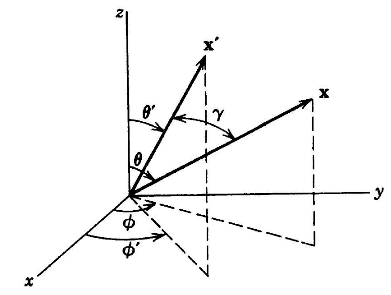
\includegraphics[scale=0.7]{Imagenes/Teorema_Adicion_01.png}
    \caption{Los dos vectores $\va{r}$ y $\va{r}^{\, \prime}$ se indican en la figura por $x$ y $\pderivada{x}$, respectivamente. El ángulo entre los dos vectores se indica por $\gamma$.}
    \label{fig:figura_01}
\end{figure}
El ángulo entre estos dos vectores, identificado por $\gamma$, se calcula fácilmente. Observando que los vectores unitarios están dados por:
\begin{align*}
\vu{r} = \sin \theta \, \cos \phi \, \vu{i} + \sin \theta \, \sin \phi \, \vu{j} + \cos \theta \, \vu{k}
\end{align*}
y de manera similar para el vector $\vu{r}^{\, \prime}$, se sigue entonces que:
\begin{align}
\cos \gamma = \va{r} \cdot \va{r}^{\, \prime} = \cos \theta \, \cos \pderivada{\theta} + \sin \theta \, \sin \pderivada{\theta} \, \cos \big( \phi - \pderivada{\phi} \big)
\label{eq:ecuacion_021}
\end{align}

El \emph{teorema de la adición para los armónicos esféricos} es:
\begin{align*}
\setlength{\fboxsep}{3\fboxsep}\boxed{
P_{\ell} (\cos \gamma) = \dfrac{4 \pi}{2 \ell + 1} \, \nsum_{m=-\ell}^{\ell} Y_{l}^{m} (\theta, \phi)^{*} \, Y_{l}^{m} (\theta, \phi) }
\end{align*}

Tengamos en cuenta que si se establece $\ell = 1$ en el teorema de la adición y se emplea $P_{1} (\cos \gamma) = \cos \gamma$, entonces el resultado coincide con la ec. (\ref{eq:ecuacion_021}). Es decir, el teorema de la adición generaliza la relación geométrica que presenta la ec. (\ref{eq:ecuacion_021}).
\par
Para probar el teorema de la suma, primero observamos que:
\begin{align}
- r^{2} \, \grad^{2} \, P_{l} (\cos \gamma) = \ell ( \ell + 1) \, P_{\ell} (\cos \gamma)
\label{eq:ecuacion_022}
\end{align}
Este resultado se justifica considerando un sistema de coordenadas en el que el eje $z$ está alineado a lo largo de $\va{r}^{\, \prime}$. En este sistema de coordenadas, $\gamma$ es el ángulo polar del vector $\va{r}$. Señalando que:
\begin{align*}
P_{\ell} (\cos \gamma) = \sqrt{\dfrac{4 \pi}{2 \, \ell + 1}} \, Y_{\ell}^{0} (\gamma, \beta)
\end{align*}
donde $\beta$ es el ángulo azimutal correspondiente en el nuevo sistema de coordenadas, se deduce que la ec. (\ref{eq:ecuacion_022}) es una consecuencia de:
\begin{align}
-r^{2} \, \grad^{2} \, Y_{\ell}^{m} (\theta, \phi) = \ell (\ell + 1) \, Y_{\ell}^{m} (\theta, \phi)
\label{eq:ecuacion_015}
\end{align}

Sin embargo, $\va{\grad}^{2}$ es un operador escalar que es invariante con respecto a las rotaciones rígidas del sistema de coordenadas. La longitud $r$ también es invariante con respecto a las rotaciones. Por tanto, la ec. (\ref{eq:ecuacion_022}) también debe ser cierto en el sistema de coordenadas original.
\par
En virtud de la ec. (\ref{eq:ecuacion_021}), $P_{\ell} (\cos \gamma)$ puede verse como una función de $\theta$ y $\phi$ (donde $\pderivada{\theta}$ y $\pderivada{\phi}$ se mantienen fijos). Por lo tanto, podemos expandir esta función en una serie de Laplace:
\begin{align}
P_{\ell} (\cos \gamma) = \nsum_{m=-\ell}^{\ell} b_{m} (\pderivada{\theta}, \pderivada{\phi}) \, Y_{\ell}^{m} (\theta, \phi)
\label{eq:ecuacion_023}
\end{align}
donde los coeficientes $b_{m}$ dependen de los parámetros fijos $\pderivada{\theta}$ y $\pderivada{\phi}$. Tomemos en cuenta que esta serie de Laplace tiene la forma:
\begin{align}
f(\theta, \phi) = \nsum_{m=-\ell}^{\ell} b_{m} \, Y_{\ell}^{m} (\theta, \phi)
\label{eq:ecuacion_019}
\end{align}
como resultado de la ec. (\ref{eq:ecuacion_022}). Resolvemos los coeficientes $b_{m}$ de la forma habitual:
\begin{align}
b_{m} (\pderivada{\theta}, \pderivada{\phi}) = \scaleint{6ex} P_{\ell} (\cos \gamma) \, Y_{\ell}^{m} (\theta, \phi)^{*} \dd{\Omega}
\end{align}
Usando la ec. (\ref{eq:ecuacion_021}), debemos evaluar:
\begin{align}
b_{m} (\pderivada{\theta}, \pderivada{\phi}) = \scaleint{6ex} P_{\ell} (\cos \theta \cos \pderivada{\theta} + \sin \theta \sin \pderivada{\theta} \cos \big[ \phi - \pderivada{\phi} \big]) \, Y_{\ell}^{m} (\theta, \phi)^{*} \dd{\Omega}
\label{eq:ecuacion_024}
\end{align}
que es difícil de calcular directamente. En su lugar, deduciremos el valor de $b_{m} (\pderivada{\theta}, \pderivada{\phi})$ con un enfoque indirecto e inteligente que evita un cálculo desordenado de una integral difícil.
\par
En el sistema de coordenadas en el que el eje $z$ se encuentra a lo largo de $\va{r}^{\, \prime}$, el vector $\va{r}$ tiene un ángulo polar $\gamma$ y un ángulo azimutal $\beta$. Los ángulos $\theta$ y $\phi$ son funciones de los ángulos $\gamma$ y $\beta$, por lo que podemos escribir la siguiente serie de Laplace:
\begin{align}
Y_{\ell m} (\theta, \phi)^{*} = \nsum_{\pderivada{m}=-\ell}^{\ell} B_{m \pderivada{m}} \, Y_{\ell \pderivada{m}} (\gamma, \beta)
\label{eq:ecuacion_025}
\end{align}
donde hemos tenido cuidado de elegir un nuevo índice mudo $\pderivada{m}$ para evitar confusiones con el índice fijo $m$. Los coeficientes $B_{m \pderivada{m}}$ se pueden determinar como de costumbre:
\begin{align*}
B_{m \pderivada{m}} = \scaleint{6ex} Y_{\ell m} (\theta, \phi)^{*} \, Y_{\ell \pderivada{m}} (\gamma, \beta)^{*} \dd{\Omega}_{\gamma}
\end{align*}
donde $\dd{\Omega}_{\gamma}$ indica el diferencial de ángulo sólido en el nuevo sistema de coordenadas. En particular, haciendo que $\pderivada{m} = 0$ y usando el resultado:
\begin{align}
Y_{\ell}^{0} (\theta, \phi) = \sqrt{\dfrac{2 \ell + 1}{4 \pi}} \, P_{\ell} (\cos \theta) \hspace{1.5cm} \ell = 0, 1, 2, \ldots
\label{eq:ecuacion_013}
\end{align}
tendremos que:
\begin{align*}
B_{m 0} = \scaleint{6ex} Y_{\ell m} (\theta, \phi)^{*} \, Y_{\ell 0} (\gamma, \beta)^{*} \dd{\Omega}_{\gamma} = \sqrt{\dfrac{2 \ell + 1}{4 \pi}} \, \scaleint{6ex} Y_{\ell m} (\theta, \phi)^{*} \, P_{\ell} (\cos \gamma) \dd{\Omega}_{\gamma}
\end{align*}
Sin embargo:
\begin{align}
\dd{\Omega}_{\gamma} = \dd{\Omega}
\label{eq:ecuacion_026}
\end{align}
dado que una rotación rígida del sistema de coordenadas deja invariante al elemento infinitesimal de ángulo sólido\footnote{Toma en cuenta que $r^{2} \dd{\Omega}$ es el área de superficie infinitesimal en una esfera de radio $r$ subtendida por el ángulo sólido infinitesimal $\dd{\Omega}$. Claramente, el área de esta superficie infinitesimal no cambia por una rotación rígida.}. Por lo tanto:
\begin{align}
B_{m 0} = \sqrt{\dfrac{2 \ell + 1}{4 \pi}} \, \scaleint{6ex} P_{\ell} (\cos \gamma) \, Y_{\ell m} (\theta, \phi)^{*} \dd{\Omega} = \sqrt{\dfrac{2 \ell + 1}{4 \pi}} \, b_{m} (\pderivada{\theta}, \pderivada{\phi})
\label{eq:ecuacion_027}
\end{align}
donde la última expresión es una consecuencia de la ec. (\ref{eq:ecuacion_024}). Sin embargo, también podemos determinar $B_{m0}$ directamente a partir de la ec. (\ref{eq:ecuacion_025}) tomando el límite cuando $\gamma \to 0$. Tengamos en cuenta que\footnote{Se puede comprobar rápidamente que $P_{\ell m} (1) = 0$ a menos que $m = 0$, en cuyo caso podemos escribir $P_{\ell}^{m} (1) = \delta_{m 0}$}:
\begin{align*}
Y_{\ell m} (0, \beta) = N_{\ell}^{m} \, P_{\ell}^{m} (1) \, e^{i  m \varphi} = \delta_{m 0} \, N_{\ell 0} = \delta_{m 0} \sqrt{\dfrac{2 \ell + 1}{4 \pi}}
\end{align*}
donde $N_{\ell m}$ es el factor de normalización en:
\begin{align}
\begin{aligned}
Y_{\ell}^{m} (\theta, \phi) = (-1)^{m} &\sqrt{\dfrac{(2 \ell +1)}{4 \pi} \dfrac{(\ell - m)!}{(\ell + m)!}} \, P_{\ell}^{m} (\cos \theta)  \, e^{i m \phi} \\[0.5em]
&\mbox{para } \begin{cases}
\ell = 0, 1, 2, \ldots \\
m = - \ell, -\ell +1, \ldots , \ell -1,  \ell
\end{cases}
\end{aligned}
\label{eq:ecuacion_09}
\end{align}

Por lo que en el límite cuando $\gamma \to 0$, el término $\pderivada{m} = 0$ de la suma en la ec. (\ref{eq:ecuacion_025}) permanece, y nos quedamos con:
\begin{align*}
\lim_{\gamma \to 0} Y_{\ell m} (\theta, \phi)^{*} = B_{m 0} \, \sqrt{\dfrac{2 \ell + 1}{4 \pi}}
\end{align*}

De esta manera, en el límite cuando $\gamma \to 0$, los vectores $\va{r}$ y $\va{r}^{\,\prime}$ coinciden, en cuyo caso $\theta \to \pderivada{\theta}$ y $\phi \to \pderivada{\phi}$. Entonces, podemos concluir que:
\begin{align*}
Y_{\ell m} (\pderivada{\theta}, \pderivada{\phi})^{*} = \sqrt{\dfrac{2 \ell + 1}{4 \pi}} \, B_{m 0}
\end{align*}
Finalmente, al sustituir $B_{m0}$ usando la ec. (\ref{eq:ecuacion_027}), llegamos a:
\begin{align*}
b_{m} (\pderivada{\theta}, \pderivada{\phi}) = \dfrac{4 \pi}{2 \ell + 1} \, Y_{\ell m} (\pderivada{\theta}, \pderivada{\phi})^{*}
\end{align*}
Ocupando este resultado en la ec. (\ref{eq:ecuacion_023}), nos lleva al teorema de adición:
\begin{align}
P_{\ell} (\cos \gamma) = \dfrac{4 \pi}{2 \ell + 1} \nsum_{m=-\ell}^{\ell} Y_{\ell}^{m} (\theta, \phi) \, Y_{\ell}^{m} (\pderivada{\theta}, \pderivada{\phi})^{*}
\label{eq:ecuacion_028}
\end{align}

\section{Una aplicación del teorema de adición.}

El inverso de la distancia entre dos vectores nos lleva a:
\begin{align}
\dfrac{1}{\abs{\va{r} - \va{r}^{\, \prime}}} = \dfrac{1}{\sqrt{r^{2} + r^{\prime 2} - 2 \, r \, r^{\prime} \, \cos \gamma}}
\label{eq:ecuacion_029}
\end{align}
donde $r \equiv \abs{\va{r}}$ y $r^{\prime} \equiv \va{r}^{\, \prime}$. En el caso de $r^{\prime} < r$:
\begin{align}
\begin{aligned}[b]
\dfrac{1}{\abs{\va{r} - \va{r}^{\, \prime}}} &= \dfrac{1}{r} \bigg( 1 + \dfrac{r^{\prime \, 2}}{r^{2}} - \dfrac{2 \, r^{\prime \, 2}}{r^{2}} \, \cos \gamma \bigg)^{-\frac{1}{2}} = \\[0.5em]
&= \dfrac{1}{r} \nsum_{\ell=0}^{\infty} \bigg( \dfrac{r^{\prime}}{r} \bigg)^{\ell} \, P_{\ell} (\cos \gamma)
\end{aligned}
\label{eq:ecuacion_030}
\end{align}
en donde en el último paso, hicimos uso de la función generatriz de los polinomios ordinarios de Legendre. En el caso de $r^\prime > r$, es suficiente intercambiar $r$ y $r^{\prime}$ en la ec. (\ref{eq:ecuacion_030}) para obtener el resultado correcto. Es conveniente introducir la notación donde $r_{<}$ es menor de las dos cantidades $r$ y $r^{\prime}$, y $r_{>}$ es la mayor de las dos cantidades $r$ y $r^{\prime}$. En ecuaciones se tendrá:
\begin{align*}
r_{<} = \min \left\{ r, r^{\prime} \right\} \hspace{1.5cm} r_{>} = \max \left\{ r, r^{\prime} \right\}
\end{align*}

Usando esta notación:
\begin{align}
\dfrac{1}{\abs{\va{r} - \va{r}^{\, \prime}}} &= \dfrac{1}{r_{>}} \nsum_{\ell=0}^{\infty} \bigg( \dfrac{r_{<}}{r_{>}} \bigg)^{\ell} \, P_{\ell} (\cos \gamma)
\label{eq:ecuacion_031}
\end{align}
la cual es convergente para todo $r \neq r^{\prime}$.
\par
Ahora invocamos el teorema de la adición de los armónicos esféricos incluyendo la ec. (\ref{eq:ecuacion_028}) para $P_{\ell} (\cos \gamma)$ en la ec. (\ref{eq:ecuacion_031}). El resultado final es la siguiente expansión para el inverso de la distancia entre dos vectores:
\begin{align}
\setlength{\fboxsep}{3\fboxsep}\boxed{
\dfrac{1}{\abs{\va{r} - \va{r}^{\, \prime}}} = 4 \pi \nsum_{\ell=0}^{\infty} \dfrac{1}{2 \ell + 1} \, \dfrac{r_{<}^{\ell}}{r_{>}^{\ell+1}} \, \nsum_{m=-\ell}^{\ell} Y_{\ell}^{m} (\theta, \phi)^{*} \, Y_{\ell}^{m} (\theta, \phi)}
\label{eq:ecuacion_032}
\end{align}
Aunque la ec. (\ref{eq:ecuacion_032}) parece bastante complicada, puede ser muy útil para evaluar ciertas integrales. Como ejemplo simple, consideremos:
\begin{align}
\scaleint{6ex} \dfrac{\dd{\Omega}}{\abs{\va{r} - \va{r}^{\, \prime}}}
\label{eq:ecuacion_033}
\end{align}
Podríamos intentar integrar directamente usando las ecs. (\ref{eq:ecuacion_021}) y (\ref{eq:ecuacion_029}):
\begin{align*}
\scaleint{6ex}_{\bs 0}^{2 \pi} \scaleint{6ex}_{\bs -1}^{1} \dfrac{\dd{\cos \theta} \dd{\phi}}{\sqrt{r^{2} + r^{\prime 2} - 2 r r^{\prime} \big[ \cos \theta \cos \pderivada{\theta} + \sin \theta \sin \pderivada{\theta} \, \cos (\phi - \pderivada{\phi}) \big]}}
\end{align*}
En realidad, es más fácil fijar primero el sistema de coordenadas de modo que $\va{r}^{\, \prime}$ se encuentre a lo largo del eje $z$. Entonces está permitido hacer que $\pderivada{\theta} = \pderivada{\phi} = 0$ sin pérdida de generalidad y evaluar:
\begin{align*}
\scaleint{6ex}_{\bs 0}^{2 \pi} \scaleint{6ex}_{\bs -1}^{1} \dfrac{\dd{\cos \theta} \dd{\phi}}{\sqrt{r^{2} + r^{\prime 2} - 2 r r^{\prime} \, \cos \theta}}
\end{align*}
Cambiando las variables a: $x = r^{2} + r^{\prime 2} - 2 r r^{\prime} \, \cos \theta$, el resultado de las integrales es elemental:
\begin{align}
\begin{aligned}[b]
\scaleint{6ex} \dfrac{\dd{\Omega}}{\abs{\va{r} - \va{r}^{\, \prime}}} &= \dfrac{\pi}{r r^{\prime}} \scaleint{6ex}_{\bs (r - r^{\prime})^{2}}^{(r + r^{\prime})^{2}} \dfrac{\dd{x}}{\sqrt{x}} = \\[0.5em]
&= \dfrac{2 \pi}{r r^{\prime}} \big( r + r^{\prime} - \abs{r - r^{\prime}} \big) = \\[0.5em]
&= \begin{cases}
\dfrac{4 \pi}{r} & \mbox{si } r > r^{\prime} \\[0.5em]
\dfrac{4 \pi}{r^{\prime}} & \mbox{si } r < r^{\prime}
\end{cases}
\end{aligned}
\label{eq:ecuacion_034}
\end{align}

Usando la ec. (\ref{eq:ecuacion_032}) se cuenta con una técnica más sencilla para evaluar la ec. (\ref{eq:ecuacion_033}):
\begin{align}
\scaleint{6ex} \dfrac{\dd{\Omega}}{\abs{\va{r} - \va{r}^{\, \prime}}} = 4 \pi \nsum_{\ell=0}^{\infty} \dfrac{1}{2 \ell + 1} \, \dfrac{r_{<}^{\ell}}{r_{>}^{\ell+1}} \, \nsum_{m=-\ell}^{\ell} Y_{\ell}^{m} (\theta, \phi)^{*} \, \scaleint{6ex} Y_{\ell}^{m} (\theta, \phi) \dd{\Omega}
\label{eq:ecuacion_035}
\end{align}
La integración sobre el ángulo sólido pues hacerse por inspección, viendo que:
\begin{align}
\sqrt{4 \pi} \, Y_{0}^{0} (\theta, \phi)^{*} = 1
\end{align}
En consecuencia, la integral sobre el ángulo sólido en la ec. (\ref{eq:ecuacion_035}), puede escribirse como:
\begin{align*}
\scaleint{6ex} Y_{\ell}^{m} (\theta, \phi) \dd{\Omega} = \sqrt{4 \pi} \scaleint{6ex} Y_{\ell}^{m} (\theta, \phi) \, Y_{0}^{0} \theta, \phi)^{*} \dd{\Omega} = \sqrt{4 \pi} \delta_{\ell 0} \, \delta_{m 0}
\end{align*}
después de usar las relaciones de ortonormalidad. Ocupando este resultado en la ec. (\ref{eq:ecuacion_035}), vemos que solo el término para $\ell = m = 0$ sobrevive. Por lo tanto, el resultado final es:
\begin{align}
\begin{aligned}
\scaleint{6ex} \dfrac{\dd{\Omega}}{\abs{\va{r} - \va{r}^{\, \prime}}} &= \dfrac{4 \pi}{r_{>}} \, \sqrt{4 \pi} ~ Y_{0}^{0} (\pderivada{\theta}, \pderivada{\phi})^{*} = \\[0.5em]
&= \dfrac{4 \pi}{r_{>}} = \\[0.5em]
&= \begin{cases}
\dfrac{4 \pi}{r} & \mbox{si } r > r^{\prime} \\[0.5em]
\dfrac{4 \pi}{r^{\prime}} & \mbox{si } r < r^{\prime}
\end{cases}
\end{aligned}
\end{align}
que reproduce de una manera más sencilla el resultado de la ec. (\ref{eq:ecuacion_034}).

% \newpage
% \section{Ejercicio a cuenta.}

% %Ref. Arfken (2006) 12.8.4 
% \noindent
% \textbf{Ejercicio a cuenta (44).} Dos protones se encuentran distribuidos \emph{uniformemente} dentro del mismo volumen esférico. Si las coordenadas de un elemento de carga son $(r_{1}, \theta_{1}, \varphi_{1})$ y las coordenadas del otro son $(r_{2}, \theta_{2}, \varphi_{2})$ y $r_{12}$ es la distancia entre ambos, el elemento de la energía de repulsión estará dado por:
% \begin{align*}
% \dd{\psi} = \rho^{2} \, \dfrac{\dd{\tau_{1}} \dd{\tau_{2}}}{r_{12}} = \rho^{2} \, \dfrac{r_{1}^{2} \dd{r_{1}} \sin \theta_{1} \dd{\theta_{1}} \dd{\varphi_{1}} \, r_{2}^{2} \dd{r_{2}} \sin \theta_{2} \dd{\theta_{2}} \dd{\varphi_{2}} }{r_{12}}
% \end{align*}
% donde:
% \begin{align*}
% \rho &= \dfrac{\mbox{carga}}{\mbox{volumen}} = \dfrac{3 \, e}{4 \, \pi \, R^{3}}, \hspace{1cm} \mbox{densidad de carga} \\[0.75em]
% r_{12}^{2} &= r_{1}^{2} + r_{2}^{2} - 2 \, r_{1} \, r_{2} \, \cos \gamma
% \end{align*}

% Demuestra que la energía electrostática total (de repulsión) de los dos protones es: $(6 \, e^{2} / 5 \, R)$.
% \par
% Este cálculo se utiliza para definir la diferencia de masa en los núcleos \enquote{a imagen de espejo}, tal como $O^{15}$ y $N^{15}$. El resultado representa el \enquote{doble} de lo requerido para crear una esfera cargada uniformemente debido a que se tienen dos cargas de nube separadas y \emph{no} una carga que interactúa consigo misma (con la permutación de los pares \emph{sin} considerar).

\end{document}